%	JASA LaTeX Sample File, Preprint Sample
%
%  Beginner Latex users should refer to their favorite online documentation
%  here is one from the TeX Users Group 
%	https://www.tug.org/twg/mactex/tutorials/ltxprimer-1.0.pdf
%
%  Useful FAQ from  https://journals.aps.org/revtex/revtex-faq
% 

%%%%%%% For Preprint
%% For manuscript, 12pt, one column style

%  \documentclass[preprint]{JASAnew}

%%%%% Preprint Options %%%%%
%% The track changes option allows you to mark changes
%% and will produce a list of changes, their line number
%% and page number at the end of the article.
%\documentclass[preprint,trackchanges]{JASAnew}

%% authaffil option will make affil immediately
% follow author, otherwise authors are grouped, and affiliations
% are stacked underneath all the authors.
%\documentclass[preprint,authaffil]{JASAnew}

%% NumberedRefs is used for numbered bibliography and citations.
%% Default is Author-Year style.
% \documentclass[preprint,NumberedRefs]{JASAnew}

%%%%%%% For Reprint
%% For appearance of finished article; 2 columns, 10 pt fonts

% \documentclass[reprint]{JASAnew}

%%%%% Reprint Options %%%%%

%% For testing to see if author has exceeded page length request, use 12pt option
% \documentclass[reprint,12pt]{JASAnew}

% authaffil option will make affil immediately
% follow author, otherwise authors are grouped, and affiliations
% are stacked underneath all the authors.
%\documentclass[reprint,authaffil]{JASAnew}

%% NumberedRefs is used for numbered bibliography and citations.
%% Default is Author-Year style.
\documentclass[reprint,NumberedRefs]{JASAnew}
\usepackage{cases}
%% TurnOnLineNumbers
%% Make lines be numbered in reprint style:
% \documentclass[reprint,TurnOnLineNumbers]{JASAnew}

\begin{document}

\title[JASA/Sample JASA Article]{The Tromba Marina: a physical modelling case study (\#superbadandpretentious)}
\author{Silvin Willemsen}
\email{sil@create.aau.dk}
\affiliation{Multisensory Experience Lab,  Aalborg University Copenhagen, Copenhagen, Denmark}
\author{Michele Ducceschi}
\author{Stefan Bilbao}
\affiliation{Acoustics and Audio Group,  University of Edinburgh, Edinburgh, Scotland}

\author{Stefania Serafin}
\affiliation{Multisensory Experience Lab,  Aalborg University Copenhagen, Copenhagen, Denmark}
 
% \author{Author Five}			% \email{author.five@someplace.edu}
% \affiliation{Department3,  University3, City, State ZipCode, Country}

\preprint{Author, JASA}		%  if you want want this message to appear in upper left corner of title page

\date{\today} 

\begin{abstract}
Put your abstract here. Abstracts are limited to 200 words for
regular articles and 100 words for Letters to the Editor. Please no
personal pronouns, also please do not use the words ``new'' and/or
``novel'' in the abstract. An article usually includes an abstract, a
concise summary of the work covered at length in the main body of the
article.     
\end{abstract}

%% pacs numbers not used

\maketitle

%  End of title page for Preprint option --------------------------------- %


\section{\label{sec:1} Introduction}
Physical modelling for sound synthesis knows a wide variety of applications\dots

Another is to make unplayable instruments, due to rarity or fragility, playable again. Our focus here is to resurrect the old and rare tromba marina. 

\subsection{History}
The tromba marina is a monochord from  \textless insert country\textgreater\ and created in ca.  \textless insert year\textgreater\ (see~\ref{fig:tromba}). It was played mainly by women. The characteristic sound of the instrument comes from the rattling bridge, that makes the instrument sound like a trumpet rather than a bowed-string instrument. 

Non-iterative collisions as presented in \cite{ducceschi2019} \dots

In \cite{bilbao2019}, the same authors have published a continuation with a focus on sonic output quality. To the best of the authors' knowledge, no other literature 


 % Sample showing how to include figure, this is a floating figure
 
\begin{figure}[ht]
%% \reprintcolumnwidth is the same in preprint and reprint for
%% ease of use for authors:
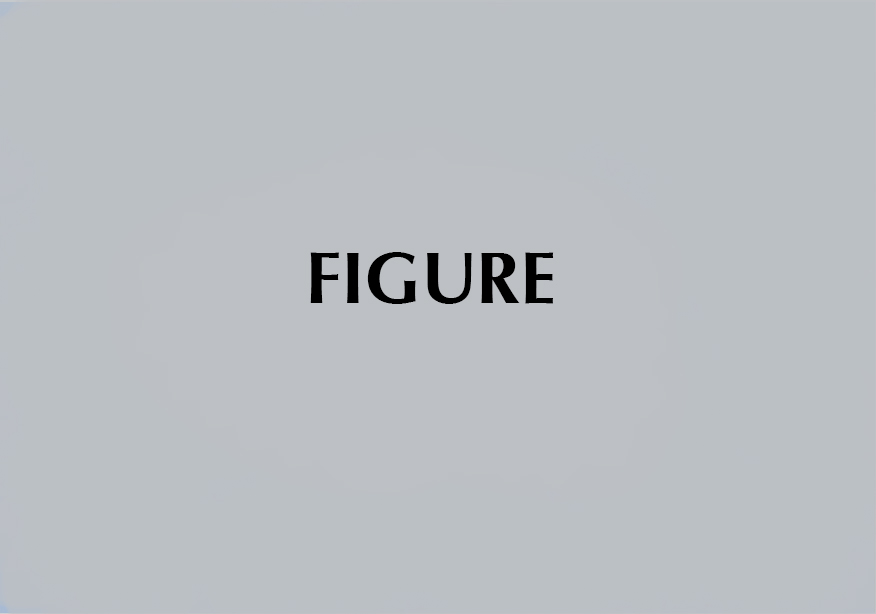
\includegraphics[width=\reprintcolumnwidth]{figsamp.jpg}
\caption{\label{fig:tromba}{The tromba marina.}}
\end{figure}

\section{\label{sec:2} Instrument design and interaction}
The tromba marina is a chordophone... The interaction with the instrument is through bowing. The string rests on a rattling bridge, causing the sound of the instrument to have brass-like qualities.
The instrument rests with the neck on the shoulder of the player and the string is bowed close to the neck -- as opposed to other bowed-string instruments which are bowed closer to the bridge. Different pitches are played by playing overtones or harmonics by placing a finger slightly on a one-over-integer multiple of the string length to create a node creating an overtone. \textit{$\Leftarrow$ Notes: need to find better wording.}

The instrument can be divided into three main components: the (bowed) string, the bridge and the body. 

\section{Models}
In this section the model equations will be presented. 
\paragraph{Notation}
Subscripts `$t$' and `$x$' denote a single derivative with respect to time or space. Furthermore, for clarity, subscripts `$\text{s}$' and `$\text{p}$' will be given for parameter symbols that are shared between the string and the plate.
\subsection{Damped Stiff String}
Using state variable $u=u(x,t)$, the motion of a damped stiff string is described as
\begin{equation}
    \rho_\text{s} A u_{tt} = Tu_{xx} - E_\text{s}Iu_{xxxx}-2\rho_\text{s}A\sigma_{0,\text{s}}u_t+2\rho_\text{s}A\sigma_{1,\text{s}}u_{txx},
\end{equation}
with material density $\rho_\text{s}$ (kg$\cdot$m$^{-3}$), cross-sectional area $A = \pi r^2$ (m$^2$), where $r$ is the string radius (m), tension $T$ (N), Young's modulus $E_\text{s}$ (Pa), area moment of inertia $I = \pi r^4 / 4$ (m$^4$) and frequency independent and dependent loss factors $\sigma_{0,\text{s}}$ (s$^{-1}$) and $\sigma_{1,\text{s}}$ (m$^2$/s).
\subsection{Bridge}
The bridge is modelled as a damped mass with a linear restoring force. Its displacement $w=w(t)$ is described as
\begin{equation}
    Mw_{tt}=-M\omega_0^2w-MRw_t,
\end{equation}
with bridge-mass $M$ (kg), angular frequency $\omega_0$ (s$^{-1}$) and damping coefficient $R$ (s$^{-1}$). The restoring force has been added to simulate the fact that\dots  It might seem odd have all terms include a multiplication with mass $M$, but as we start adding the effects of other parts of the system, it will make more sense.
\subsection{Body}
For simplicity, the body is modelled as a 2D plate. The displacement $v = v(x,y,t)$ at location $(x,y)$ is described as
\begin{equation}
    \rho_\text{p} H v_{tt}=-D\Delta\Delta v-2\sigma_{0,\text{p}}v_t+2\sigma_{1,\text{p}}\Delta v_t,
\end{equation}
with material density $\rho_\text{p}$ (kg$\cdot$m$^3$), plate thickness $H$ (m), $D = E_\text{p}H^3/12(1-\nu^2)$ (kg$\cdot$m$^2\cdot$s$^{-2}$), where $E_\text{p}$ is the Young's modulus (Pa) and $\nu$ the unitless Poisson's ratio, and and frequency independent and dependent loss factors $\sigma_{0,\text{p}}$ (s$^{-1}$) and $\sigma_{1,\text{p}}$ (m$^2$/s). Furthermore, $\Delta$ represents the 2D Laplacian and is defined as
\begin{equation}
    \Delta = \frac{\partial^2}{\partial x^2} + \frac{\partial^2}{\partial y^2}.
\end{equation}
\subsection{Implementation}
The complete system is shown in Eqs.~(\ref{eq:systemString}) --~(\ref{eq:systemEtaSpring}).
\begin{subnumcases}{\label{eq:trombaSystem}}
    \begin{aligned}&\rho_\text{s} A \delta_{tt}u^n_l\\
    &\\ & \end{aligned} & $\!\!\!\!\!\!\!\!\!\!\begin{aligned}=&\ T\delta_{xx}u^n_l - E_\text{s}I\delta_{xxxx}u^n_l \\
        &- 2\rho_\text{s}A\sigma_{0,\text{s}}\delta_{t\cdot}u^n_l\\
        &+2\rho_\text{s}A\sigma_{1,\text{s}}\delta_{t-}\delta_{xx}u^n_l-J_\text{s}(l_\text{br})F_\alpha\end{aligned}\quad\ \ $\label{eq:systemString} \\
        \begin{aligned}
        &M \delta_{tt}w^n\\
        &
    \end{aligned} &$\!\!\!\!\!\!\!\!\!\!
        \begin{aligned}=&-M\omega_0^2w^n - MR \delta_{t\cdot}w^n\\
            & + \big(\mu_{t+}\psi^{n-1/2}\big)g^n + F_\alpha
        \end{aligned}$\\
    \begin{aligned}
    &\rho_\text{p} H \delta_{tt}v^n_{(l,m)}\\ 
    & \\
    &
    \end{aligned}
    & $\!\!\!\!\!\!\!\!\!\!\begin{aligned} 
    =&-D\delta_{\Delta \boxplus}\delta_{\Delta \boxplus}v_{(l,m)}^n - 2\sigma_{0, \text{p}}\delta_{t\cdot}v^n_{(l,m)}\\
    &%\!\!\!\!\!\!\!\!\!\!\!\!\!\!\!\!\!\!\!\!\!\!\!\!\!\!
    + 2\sigma_{1, \text{p}}\delta_{t-}\delta_{\Delta\boxplus}v_(l,m)^n\\
    & - J_\text{p}(l_\text{br},m_\text{br}) \big(\mu_{t+}\psi^{n-1/2}\big)g^n
    \end{aligned}$\\
\begin{aligned}
\delta_{t+}\psi^{n-1/2} 
\end{aligned}
&$\!\!\!\!\!\!\!\!\!\!
\begin{aligned}= g^n\delta_{t\cdot}\eta_\text{c}^n
\end{aligned}$\\
\begin{aligned}
    \eta_\text{c}^n 
\end{aligned}
&$\!\!\!\!\!\!\!\!\!\!
\begin{aligned}
    = v_{(l_\text{br},m_\text{br})}^n - w^n
\end{aligned}$\\
    \begin{aligned}
        &F_\alpha \\
        &
    \end{aligned}
    & $\!\!\!\!\!\!\!\!\!\!
    \begin{aligned}
        =&\ K_1\mu_{tt}\eta_\text{sp}^n + K_3(\eta_\text{sp}^n)^2\mu_{t\cdot}\eta_\text{sp}^n \\
        &+ 2 \sigma_\times\delta_{t\cdot}\eta_\text{sp}^n
    \end{aligned}$\label{eq:fAlphaDamp}\\
\begin{aligned}\eta_s^n\end{aligned} &$\!\!\!\!\!\!\!\!\!\!
\begin{aligned}
    = u_{l_\text{br}}^n - w^n
\end{aligned}$\label{eq:systemEtaSpring}
\end{subnumcases}
% \begin{subnumcases}{\label{eq:trombaSystem}}
%     \rho_\text{s} A \delta_{tt}u^n_l & $\!\!\!\!=T\delta_{xx}u^n_l - EI\delta_{xxxx}u^n_l - J_\text{s}(l_\text{br})F_\alpha\qquad\quad$ \\
%     M \delta_{tt}w^n &$\!\!\!\!=-M\omega_0^2w^n + \big(\mu_{t+}\psi^{n-1/2}\big)g^n + F_\alpha\qquad\quad$\\
%     \begin{aligned}&\rho_\text{p} H \delta_{tt}v^n_{(l,m)}\\ 
%     & \end{aligned} & $\!\!\!\!\!\!\!\,\,\begin{aligned} =&-D\delta_{\Delta \boxplus}\delta_{\Delta \boxplus}v_{(l,m)}^n \\
%     &- J_\text{p}(l_\text{br},m_\text{br}) \big(\mu_{t+}\psi^{n-1/2}\big)g^n \end{aligned}$\\
%     \delta_{t+}\psi^{n-1/2} &$\!\!\!\!= g^n\delta_{t\cdot}\eta_\text{c}^n$\\
%     \eta_\text{c}^n &$\!\!\!\!= v_{(l_\text{br},m_\text{br})}^n - w^n$\\
%     F_\alpha & $\!\!\!\!= K_1\mu_{tt}\eta_\text{s}^n + K_3(\eta_\text{s}^n)^2\mu_{t\cdot}\eta_\text{s}^n$\label{eq:fAlpha}\\
%     \eta_s^n &$\!\!\!\!= u_{l_\text{br}}^n - w^n$\label{eq:etaSpring}
% \end{subnumcases}
\\
%
The time-difference operators have been chosen so that the system is as accurate as possible while still being explicit 

{\bfseries\itshape
Compare the results you get with\\
{\verb+\documentclass[preprint]{JASAnew}+ }\\
vs.\\
{\verb+\documentclass[preprint,NumberedRefs]{JASAnew}+ }
}

\bibliography{sampbib}


\end{document}




